
\chapter{The RespVis Library}
\label{chap:RespVis}

RespVis is an open-source \parencite{RespVisGitHub} D3 extension
library for creating responsive SVG charts \parencite{RespVisLive}. It
enables the use of CSS for the responsive styling and layout of
visualizations. RespVis renders visualizations as pure and complete
SVG documents, meaning that the whole visualization is contained in
one SVG document and includes no elements of other XML namespaces.
RespVis is designed as an extension to D3, rather than a wrapper
around it. Unlike most other visualization libraries built on top of
D3, RespVis does not hide it behind a custom API. Rather,
visualization authors invoke RespVis functionality by binding
specially structured data to D3 Selections, which render visualization
components using render functions to transform the bound data into
some form of visual representation. Furthermore, RespVis espouses the
strong separation between data and code and applies strong static
type-checking through the use of TypeScript.





\section{Design}
\label{sec:Design}

The design of the RespVis library is guided by six principles:
\begin{enumerate}
\item Style and Layout via CSS.
\item Pure and Complete SVG Documents.
\item Extend D3.
\item Separate Data and Code.
\item Strong Static Type-Checking with TypeScript.
\item Layered Component Hierarchy.
\end{enumerate}



\subsection{Style and Layout via CSS}

Every part of a visualization that can be configured with CSS should
be configured with CSS. The visual appearance and layout of HTML
elements can already be configured by CSS. Many presentation
attributes of SVG elements can also be styled with CSS. However,
CSS-based layouting cannot be applied to SVG elements, which seriously
limits the responsive capabilities of using CSS for SVG charts.
Without powerful CSS layout technologies like Flexbox and Grid, all
the individual components of an SVG chart have to be positioned
manually via JavaScript.

The RespVis Layouter enables the layouting of visualization
components using powerful CSS-based layout mechanisms such as Flexbox and Grid, by calculating
the bounding boxes of SVG elements from the CSS configuration of a
shadow \elname{<div>} hierarchy. The Layouter offers visualization
authors comparable configurability to what they are used to when
laying out HTML elements. For example, a legend can be configured to
be placed to the right of a chart in a wider view, and beneath the
chart in a narrower view, using familiar CSS constructs.





\subsection{Pure and Complete SVG Documents}

Every RespVis visualization should be rendered as a pure and complete
SVG document. An SVG document is considered \emph{pure}, if it
contains only elements defined in the SVG namespace. This means that
it must not contain any \elname{<foreignObject>} elements, which embed
elements of an XML namespace other than SVG, for example to embed HTML
elements inside an SVG. RespVis does not support rendering to HTML
canvas elements, because graphics rendered there cannot be styled by
CSS.

An SVG document representing a visualization is considered
\emph{complete}, if it contains the entire visualization within
it. Splitting visualization components across multiple SVG documents
is considered bad practice, because these components conceptually
belong together and should be represented as a whole. Having
a full visualization enclosed in a complete SVG document allows the
whole visualization to be exported and stored as a standard-compliant
SVG file, which can be further processed using a wide range of tools.




\subsection{Extend D3}

RespVis is designed as a library which extends D3, rather than a
wrapper around D3. Compared to other visualization libraries which
wrap a layer around D3, it does not provide an entirely new interface
to visualization authors, but uses D3 Selections as the core interface
with which to interact. The typical workflow of invoking RespVis
functionality is to bind data objects of a specific structure to the
elements of a Selection and then to visualize this data by calling a
render function to transform it into visual marks. If D3 were hidden
behind a custom API, its powerful capabilities would not be directly
accessible to users of the library, and would need to be exposed
manually through special mechanisms. By designing RespVis as an
extension of D3, visualization authors can continue to leverage its
expressive and concise API and author their documents using data joins
and the general update pattern.



\subsection{Separate Data and Code}

In RespVis, data and code are decoupled from each other. Everything in
RespVis is built from functions and objects without using any classes.
Classes were avoided, since they are not common when working with D3,
and also because they lead to a tight coupling between data and
functionality, which was deemed undesirable. The decoupling of data
and code results in various benefits compared to the prevalent
object-oriented way of building software. Among these benefits are
easier reuse and testing of functions and a software system which
requires less cognitive effort to understand.

Functions are easier to reuse because they only require well-shaped
input data to perform their task. Mechanisms like inheritance or
composition, which tend to increase the complexity of a system, are
unnecessary. Compared to class-based code, where an object needs to be
instantiated before testing its methods, it is easier to test
functions in isolation when they are not coupled to their data. The
reason for this is that the instantiation of an object might be a
complex operation dependent on other methods which could affect the
results of a test case.

Possibly the main benefit of decoupling data and code lies in the
reduced complexity of the resulting system. A software system which
treats data and code as different entities might be composed of more
entities than a system which does not, but the individual entities
have fewer dependencies between one another. The reduced number of
dependencies between entities results from separating entities into a
data entities group and a function entities group, with no
relationships between them. The research related to software
complexity is hard to convey in simple terms, but one rule of thumb is
well summarized by \textcite{DataCodeSeparation} as \enquote{A system
  made of disjoint simple parts is less complex than a system made of
  a single complex part.} Of course, there are also drawbacks when
designing a system adhering to this concept, but they are not too
severe and are therefore not listed here. For further reading on this
topic, the reader is directed to Moseley and Marks' classic workshop
paper \parencite{OutOfTarPit} and Sharvit's forthcoming book
\parencite{Sharvit-Book}.




\subsection{Strong Static Type-Checking with TypeScript}

The RespVis library is written in TypeScript, with everything being as
strongly-typed as possible. For the most part, interfaces are used to
describe the structure of data objects, and function parameters are
annotated with types. Whenever working with D3 Selections, their
contents are typed as strongly as possible using the generic type
variables available on Selections. Most of the time, it is sufficient
to specify only the type of elements contained in a Selection and the
structure of the data bound on them. If the element and data types of
a Selection are declared, the various functions can assume that
parameters passed to them have specific types, and they do not have to
worry about dynamic type checking. Applying a strongly typed system
has many advantages, such as better development tooling and
compile-time identification of type-related bugs. These advantages
have already been described in Section~\ref{sec:TS}.







\subsection{Layered Component Hierarchy}

Components in RespVis are structured in four layers with increasing
levels of abstraction, as shown in Figure~\ref{fig:Layers}. Components
in higher layers make more assumptions about their content than
components in lower layers. The bottom-most layer with the lowest
level of abstraction consists of visual Primitives, represented by
basic SVG elements like \elname{<rect>}, \elname{<circle>}, and
\elname{<text>}. These Primitives do not require any data to be bound to
them and are simply rendered by setting their attributes to the
desired values.


\begin{figure}[tp]
\centering
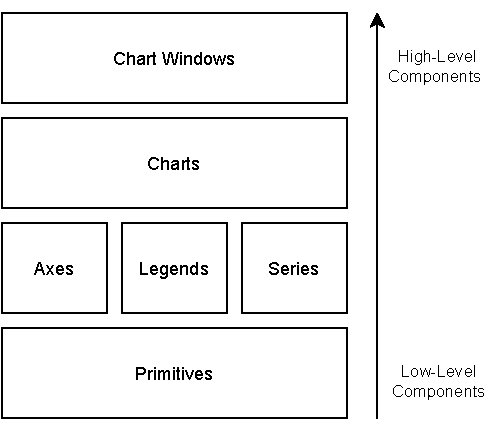
\includegraphics[keepaspectratio,width=\linewidth,height=7.5cm]
{diagrams/respvis-layers.pdf}
\caption[Component Layers of RespVis]{
The four layers of components in the RespVis library. Higher layers
contain increasingly higher-level components.
\imgcredit{Image created by the author of this thesis.}
}
\label{fig:Layers}
\end{figure}


The second layer comprises composite components such as Axes, Legends,
and Series. These are usually rendered as \elname{<svg>} or \elname{<g>}
elements containing only primitive elements. The components in this
layer are the lowest-level components which are configured using
structured data bound to their elements. Series components are
composite elements which render a collection of underlying elements
using a data join and the general update pattern.

The third layer consists of Chart components. Charts are composite
components which can also include other composite components. They are
the visual entities which represent complete visualizations and are
usually composed of axes, series, and legends.

In many other visualization libraries, charts are the highest-level
components visualization authors can work with, but RespVis contains
an additional layer above them, formed by Chart Window components.
Chart Windows are wrapper components around Charts. Unlike the
previously discussed lower layers, Chart Windows are not rendered as
SVG elements but as HTML \elname{<div>} elements. Their purpose is to
nest Charts into a Layouter component, render them in a three-phased
rendering process, and provide an optional toolbar for them. Toolbars
are customizable and can hold different tools for different types of
chart.








\section{Naming Conventions}
\label{sec:NamingConventions}

The naming of entities in RespVis follows the same naming conventions
used in D3 modules. The names of entities usually start with the name
of the group to which an entity belongs and are then further narrowed
down by successively adding more words until the exact entity is
accurately described. This convention is referred to as
\enquote{top-down naming} in this thesis. An example of the top-down
naming convention can be seen in the D3 Scale
\parencite{D3Scale} and D3 Axis \parencite{D3Axis} packages, in
which entities are called things like \code{scaleLinear},
\code{scaleOrdinal}, \code{axisBottom}, and \code{axisLeft} rather
than \code{linearScale}, \code{ordinalScale}, \code{bottomAxis}, and
\code{leftAxis}. Since this is the exact opposite of how these
entities would be called in natural English, using such names
can feel odd for the uninitiated. However, experience shows working
with APIs which follow such a naming convention is easier than with
those which do not, since users of such APIs can easily discover
specialized entities by inputting the general entity type and browsing
through code completion suggestions provided by their development
tools. Hence, entity names in RespVis also follow this convention.

RespVis' public interface is made up of types and functions. Types
are usually written as interfaces and represent the shape of an
object. Type names are written in \code{PascalCase}
\parencite{PascalCase} and adhere to the top-down naming
convention. They always start with the group a type belongs to, and
further words are appended to distinguish ever more specialized
types. The naming of types can best be demonstrated by the different
names given to interfaces describing data objects to configure
different kinds of Bar Charts. Data objects for the configuration of
Basic Bar Charts are described by the \code{ChartBar} interface, those
of Grouped Bar Charts are described by the \code{ChartBarGrouped}
interface, and those of Stacked Bar Charts are described by the
\code{ChartBarStacked} interface.

The API of RespVis is largely composed of functions. Function names
are always written in \code{camelCase} \parencite{camelCase} and also
follow the top-down naming convention. Function names always start
with the type of object on which they operate, followed by the
operation they perform. A component in RespVis always consists of a
data object which describes it, an element to which the data object is
bound, and a render function which transforms the bound data into some
form of visual representation. The names of functions to create data
objects for the configuration of components are always in the form of
\code{componentNameData}, such as \code{chartBarData} or
\code{chartBarGroupedData}. Functions which transform bound data into
a visual representation are always named in the form of
\code{componentNameRender}, such as \code{chartBarRender} or
\code{chartBarGroupedRender}.






\section{Project Structure}
\label{sec:ProjectSetup}

RespVis is a NodeJS \parencite{NodeJS} project hosted as an
open-source project on GitHub \parencite{RespVisGitHub}. It is
implemented in TypeScript and grouped into different packages by
thematic affinity. The TypeScript source files are compiled
(transpiled) to JavaScript and bundled into one combined library
package, which visualization authors can then import into their
projects.
%
The Rollup module bundler \parencite{Rollup} is used to perform
compilation and bundling. In addition to the bundled JavaScript
library, visualization authors are required to import an accompanying
CSS file containing default styling for the generated visualizations.
The project also contains examples demonstrating usage of the library
to create various charts. These examples are HTML files which import
the required files and contain JavaScript to invoke RespVis
functionality to create and update visualizations.
%
The Gulp \parencite{Gulp} task runner is used to automate the build
process of the library, including the preparation of the output
directory, the bundling of library code, and the copying of various
files to the correct locations in the output directory.




The RespVis project contains configuration files for various tools, a
\code{src/} directory containing the source code for the whole library
and accompanying examples, a \code{node_modules} directory containing
the project's cached NodeJS dependencies, and a \code{dist/} directory
containing built versions of the library and examples ready for
distribution. The configuration files are only discussed broadly here,
later sections go into more detail about the setup of the various
tools. An overview of the most important files and directories can be
seen in Figure~\ref{fig:RespVisDirTree}.

\begin{figure}[tp]
\centering
\framebox[\textwidth]{%
\begin{minipage}{0.9\textwidth}
\begin{footnotesize}
  \dirtree{%
  .1 /.
  .2 dist/.
  .3 examples/.
  .4 data/.
  .4 vendor/.
  .4 bar.html.
  .4 \dots.
  .3 index.html.
  .3 respvis.css.
  .3 respvis.[m]js.
  .3 respvis.[m]js.map.
  .3 respvis.min.[m]js.
  .3 respvis.min.[m]js.gz.
  .3 respvis.min.[m]js.map.
  .2 node\_modules.
  .2 src/.
  .3 lib/.
  .4 bars/.
  .4 core/.
  .4 legend/.
  .4 lines/.
  .4 points/.
  .4 tooltip/.
  .3 examples/.
  .4 data/.
  .4 vendor/.
  .4 bar.html.
  .4 \dots.
  .3 index.html.
  .3 respvis.css.
  .2 gulpfile.js.
  .2 package.json.
  .2 tsconfig.json.
  }
\end{footnotesize}
\end{minipage}
}
\caption[RespVis Directory Structure]{
  The most important files and directories of the RespVis project. 
  \imgcredit{Figure created by the author of this thesis.}
}
\label{fig:RespVisDirTree}
\end{figure}


The root directory of the RespVis project contains the necessary
project configuration files for NodeJS, TypeScript, and Gulp. The
NodeJS configuration file, \code{package.json}, describes the
meta-data of the NodeJS package. It is used to specify the project's
dependencies to other packages and is required for every NodeJS
package so that it can be uploaded to the npm package registry
\parencite{npm}. The TypeScript configuration file,
\code{tsconfig.json}, specifies the configuration the TypeScript
compiler uses to compile the library's TypeScript source files into
their JavaScript counterparts. The Gulp configuration file,
\code{gulpfile.js}, is used to describe atomic, recurring tasks and
compositions of them. These tasks can then be invoked via the Gulp
command-line tool to automate otherwise tedious workflow processes.

The \code{src/} directory at the root of the project contains all the
implementation files of the library in the \code{src/lib/} directory
and examples in the \code{src/examples/} directory. The
\code{src/lib/} directory contains all TypeScript source files of the
library. They are partitioned into packages formed around the thematic
affinity of the various components. The Core package
contains the core functionality of the library and is a prerequisite
for all the other packages. It includes the Layouter, Chart base
functionality, Chart Window base functionality, and various utility
functions. The Legend package contains modules to render
legends consisting of a title and configurable labeled symbols. The
Tooltip package contains functions to show and hide
tooltips, modify their contents, and position them. It also contains
helper functions for Series to prevent the replication of
tooltip-related code in their data creation and rendering functions.
The Bars, Lines, and Points packages
contain the necessary modules to render Series, Charts, and Chart
Windows for bar, grouped bar, stacked bar, line, and point
visualizations. At the moment, all these packages are built into a
combined one, but there are plans to also distribute them separately
to allow users of the library to import only the packages they need.

The \code{src/examples/} directory holds the source files of the
developed examples. These examples are distributed alongside the
library files, and are copied over to the \code{dist/examples/}
directory when building the project. Every example consists of an HTML
file which imports all the requirements such as \code{respvis.js} and
\code{respvis.css} as well as external dependencies such as D3. It
then invokes the necessary RespVis functionality within a
\elname{<script>} tag embedded in the body of the HTML document. In
addition to individual example files, the \code{examples} directory
also contains a \code{vendor} directory, which contains third-party
dependencies, and a \code{data} directory containing data imported by
individual examples.

In addition to configuration files and the \code{src/} directory, the
root directory also contains two directories which are automatically
generated during the build process. These are the \code{node_modules/}
and \code{dist/} directories. The \code{node_modules/} directory
exists in every NodeJS package. It is created when installing the
dependencies of a package and contains a cached copy of every
direct and indirect dependency. The \code{dist/} directory is
generated by the Gulp build tasks and contains all the files necessary
to distribute a built version of the RespVis library.

The code of RespVis is distributed as JavaScript bundles in different
formats which can be used depending on the situation. These formats
are based on both Immediately Invoked Function Expressions (IIFE) and
the more modern ES modules format, both of which are explained in more
detail in Section~\ref{sec:Rollup}. Bundles containing the \code{.js}
extension in their file name contain IIFE source code, whereas bundles
containing the \code{.mjs} extension contain ES module source code.
Furthermore, these bundles are also distributed in minimized versions.
The \code{dist/respvis.[m]js} file contains the unmodified JavaScript
bundle that can be used by library consumers who require readable
code, \code{dist/respvis.min.[m]js} contains the minified JavaScript
bundle, and \code{dist/respvis.min.[m]js.gz} contains the minified
JavaScript bundle that has additionally been compressed in the GZIP
format \parencite{GZIP}. Alongside these code bundles, Rollup creates
source maps for the \code{dist/respvis.[m]js} and
\code{dist/respvis.min.[m]js} bundles: \code{dist/respvis.[m]js.map}
and \code{dist/respvis.min.[m]js.map}, respectively. These source maps
are interpreted by developer tools in browsers to map from certain
instructions in the bundled JavaScript code to the exact instruction
in the original TypeScript code and are immensely helpful for
debugging.

Since RespVis aims to perform all possible styling in CSS, the
distribution also contains a \code{dist/respvis.css} file with the
default styles for visualizations created with RespVis. Currently,
this file is written manually as a whole in the \code{src/} directory
and merely copied to the \code{dist/} directory during the build
process. In the future, this process could be improved by employing a
CSS preprocessing tool such as SASS \parencite{SASS}, so that the
styles can be split into multiple files during development. Besides
the bundled library source code and stylesheet, the \code{dist/}
directory also contains usage examples of RespVis in the
\code{dist/examples/} directory, copied over from the
\code{src/examples/} directory.






\section{NodeJS}

NodeJS is a standalone JavaScript runtime \parencite{NodeJS}, built on
top of the V8 JavaScript engine \parencite{V8}, which is an
open-source and multi-platform runtime for the execution of JavaScript
code. NodeJS allows JavaScript code to be run outside of web browsers.
NodeJS is heavily used for server-side development to unify the
technology stack of web developers and allow them to use JavaScript
for both client-side and server-side development. However, with the
appropriate project setup, NodeJS can be used for any kind of
development, and it can be set up as a powerful framework to develop
client-side applications as done in this project. One of the most
important tools in the NodeJS environment is the npm package manager
\parencite{npm}, which exists to simplify the sharing of packages and
their dependency management. The npm package registry hosts a huge
number of packages that can easily be imported and used to create new
ones.

RespVis is developed as an npm package. Every npm package is
configured via a \code{package.json} file. This file contains all the
necessary meta-data for a package to make it identifiable and provide
information about what the package contains. The \code{package.json}
file also lists all the dependencies of a package, so they can
automatically be updated and downloaded during an installation
process. A package can rely upon both normal dependencies and
development dependencies. Normal dependencies of a package are
required for it to work at run time and need to be installed alongside
it. Development dependencies are only required during development and
are only installed when installing a local package. The
\code{package.json} file is located in the root directory of the
RespVis package and can be seen in Listing~\ref{list:PackageJSON}.


\begin{samepage}
\lstinputlisting[%
  float=tp,
  aboveskip=\floatsep,
  belowskip=\floatsep,
  xleftmargin=0cm,              % no extra margins for floats
  xrightmargin=0cm,             % no extra margins for floats
  %
  basicstyle=\footnotesize\ttfamily,
  frame=shadowbox,
  numbers=left,
  label=list:PackageJSON,
  caption={[RespVis \code{package.json} File]%
    The \code{package.json} file of the RespVis library.
    This file contains all the meta-data describing the package and its dependencies.
    Keywords and type dependencies have been omitted for readability.
  },
]{listings/package.json}
\end{samepage}





\section{Rollup}
\label{sec:Rollup}

The Rollup module bundler \parencite{Rollup} is used to bundle the
source code of the RespVis library into bundles of different
kinds. Bundling combines code written as multiple smaller modules into
one combined package to make it easier to distribute. Developers do
not have to worry about the details of how their code will be
packaged, as Rollup takes care of all the necessary
transformations. In addition to bundling source code, Rollup also
performs \emph{tree shaking} on the bundled code, eliminating unused
code from the resulting bundle by statically analyzing dependencies
between modules.
%
Rollup supports the creation of bundles in several common module
formats, such as CommonJS, Asynchronous Module Definition (AMD),
Universal Module Definition (UMD), Immediately Invoked Function
Expressions (IIFE), and ES. RespVis is distributed as both IIFE and ES
modules.

IIFE modules have been used for a long time, as they were used to
support modular software designs in JavaScript before more elaborate
module formats were defined. They are anonymous functions which are
executed directly after declaring them. These functions contain the
full logic of the module and return an object representing its
publicly accessible interface. This object is usually stored in a
variable to allow interactions with the module after its creation.
IIFE modules are plain JavaScript and do not require any modern
features to be supported by browsers. They are simply loaded in web
documents like any other JavaScript resource via a \elname{<script>}
element. The example in Listing~\ref{list:IIFE} illustrates the IIFE
module format.



\begin{samepage}
\lstinputlisting[%
  float=tp,
  aboveskip=\floatsep,
  belowskip=\floatsep,
  xleftmargin=0cm,              % no extra margins for floats
  xrightmargin=0cm,             % no extra margins for floats
  %
  basicstyle=\footnotesize\ttfamily,
  frame=shadowbox,
  numbers=left,
  label=list:IIFE,
  caption={[IIFE Module Format]%
Immediately Invoked Function Expression (IIFE) modules wrap the module
code inside a function which is executed immediately after declaring it
and returns the public interface of the module.
\code{do-something.js} contains the original code that should be
wrapped as an IIFE module, \code{module.js} contains the code of the
IIFE module, and \code{application.js} demonstrates usage of the
module.
},
]{listings/iife.js}
\end{samepage}



ES modules are a more recent addition to JavaScript, introduced in
ECMAScript 6 \parencite{ECMAScript6}. They are a native module system
built around the \code{import} and \code{export} statements, which are
widely supported by modern browsers. Since the individual modules of
the RespVis library are built as ES modules anyway, Rollup mostly only
has to merge them to create a valid, combined ES module. ES modules
are natively supported in browsers, so they can be loaded directly in
a HTML document using a \elname{<script>} element. However, it is
necessary to mark them as modules by setting the \attrname{type}
attribute to \code{module} on the loading \elname{<script>} element,
so that browsers can interpret them accordingly.


The core package of Rollup is only able to create mostly unmodified
bundles from JavaScript source files. Various plugins add
frequently required additional functionality. There are two kinds of
Rollup plugins: bundle plugins, which affect the bundling process, and
output plugins, which transform the already bundled code.

The Rollup bundle plugins used for the bundling of RespVis are
\code{@rollup/plugin-node-resolve}, \code{@rollup/plugin-commonjs},
and \code{@rollup/plugin-typescript}. The
\code{@rollup/plugin-node-resolve} plugin is used to resolve imports
from other NodeJS packages that reside in the \code{node_modules}
directory. Since many NodeJS packages are still implemented as
CommonJS modules, which are not natively supported by Rollup, the
\code{@rollup/plugin-commonjs} plugin is used to interpret them.
Lastly, the \code{@rollup/plugin-typescript} plugin is used to compile
TypeScript source files to JavaScript before bundling them. The
configuration for the TypeScript compiler is taken from the
\code{tsconfig.json} file at the root directory of the project.

The Rollup output plugins used during the bundling process are
\code{rollup-plugin-terser} and \code{rollup-plugin-gzip}. These
plugins do not affect every created bundle, but are used to
selectively transform the contents of specific bundles. The
\code{rollup-plugin-terser} plugin is used to create minified versions
of the RespVis bundles denoted by the term \code{.min} in their file
names. Logically, they are equivalent to non-minified bundles, but are
compressed as much as possible to reduce their file size while still
containing valid, but unreadable, JavaScript code. The
\code{rollup-plugin-gzip} plugin is used to create compressed gzipped
versions of the RespVis bundles denoted by the term \code{.gz} in
their file extensions \parencite{GZIP}.

Note that D3 is not included in any of the generated RespVis
bundles. RespVis is designed to be an extension of D3 and, most of the
time, an application wishing to use RespVis will already be using
D3. If D3 were to be included in the RespVis bundle, it would
unnecessarily be loaded a second time. To prevent D3 from being
included in the created bundles, all dependencies on D3-related
packages are marked as external.

The actual bundling is performed via the JavaScript API of Rollup in
the private \code{bundleJS} Gulp task. This task is executed in
various automation processes set up with Gulp, which are explained in
more detail in Section~\ref{sec:Gulp}. The code of the \code{bundleJS}
task can be seen in Listing~\ref{list:BundleJS}. The RespVis library
is bundled via the \code{Rollup.rollup} function which returns the
created bundle. This bundle is then written to one or more target
destinations via the \code{Bundle.write} method, which allows the
specification of the target bundle format and any plugins used to
transform the code before writing it.


\begin{samepage}
\lstinputlisting[%
  float=tp,
  aboveskip=\floatsep,
  belowskip=\floatsep,
  xleftmargin=0cm,              % no extra margins for floats
  xrightmargin=0cm,             % no extra margins for floats
  basicstyle=\footnotesize\ttfamily,
  frame=shadowbox,
  numbers=left,
  label=list:BundleJS,
  caption={[Gulp Task to Bundle RespVis]%
The private Gulp task which bundles the code of the RespVis libary.
The bundle is created once and then written to multiple targets.
}
]{listings/bundle-js.js}
\end{samepage}
  





\section{Gulp}
\label{sec:Gulp}

Gulp is a task runner which automates workflow processes via a set of
named tasks \parencite{Gulp}. It is used to automate processes like
building the library and serving examples on a development server.
Tasks are useful for automating operations which need to be carried
out repeatedly. They can perform an atomic operation or be composed of
other tasks. Composite tasks can execute tasks contained in them in
serial or in parallel. The tasks are implemented as JavaScript
functions in the Gulp configuration file, \code{gulpfile.js}, which
can be found in the root directory of the project. Gulp's approach of
favoring code over declarative configuration files means that the
person setting up process automation needs to be familiar with
JavaScript. In return, the possibilities of configuration are endless.

Tasks in the \code{gulpfile.js} file are separated into private and
public tasks. Private tasks are simply asynchronous functions which
perform a certain action that does not necessarily have to be executed
by external entities. The private tasks in the RespVis project are
\code{bundleJS}, \code{bundleCSS}, \code{copyExamples},
\code{cleanDist}, \code{cleanNodeModules}, and \code{reloadBrowser}.
%
Public tasks are also asynchronous functions, but they are exported
and are therefore available to be executed via the Gulp command-line
interface. Most public tasks in the RespVis project are compositions
of other tasks. The public tasks in RespVis are \code{clean},
\code{cleanAll}, \code{build}, and \code{serve}. The default task,
\code{serve}, is executed when no other task is specified on the
command line. A hierarchical representation of all the tasks in the
\code{gulpfile.js} file is shown in Listing~\ref{list:GulpTasks}.

\begin{samepage}
\lstinputlisting[%
  float=tp,
  aboveskip=\floatsep,
  belowskip=\floatsep,
  xleftmargin=0cm,              % no extra margins for floats
  xrightmargin=0cm,             % no extra margins for floats
  %
  basicstyle=\footnotesize\ttfamily,
  frame=shadowbox,
  numbers=left,
  label=list:GulpTasks,
  caption={[Tasks Defined in \code{gulpfile.js}]%
A hierarchical representation of the tasks defined in the \code{gulpfile.js} file,
as output by the \code{gulp --tasks} command.
},
]{listings/gulp-tasks.txt}
\end{samepage}
  


Bundling the RespVis library's source code is implemented in the
private \code{bundleJS} task. It uses the JavaScript API of Rollup to
compile the TypeScript source files into JavaScript and bundle them
into IIFE and ES modules of varying levels of minification. This task
has already been described in detail in Section~\ref{sec:Rollup}, so
it won't be discussed further here. It is executed during the public
\code{build} and \code{serve} tasks.

The \code{bundleCSS} task is used to copy the \code{src/respvis.css}
file to the \code{dist/} directory. Since one of the design pillars of
RespVis is to style everything possible with CSS, this file contains
all the default styles for visualizations created with
RespVis. Currently, this file is one large single file in the
\code{src/} directory and is merely copied over to the \code{dist/}
directory, but there are plans to build this file from different
modules using a CSS preprocessor in the future, which will require an
additional bundling step. This task is executed as part of the public
\code{build} and \code{serve} tasks.

The private \code{copyExamples} task copies all the files from the
\code{src/examples/} directory to the \code{dist/} directory. This
task is required because the examples are developed inside the
\code{src/} directory, but need to be made available in the
distributable library packages. Another reason for the copying is that
the BrowserSync development server is initialized with the
\code{dist/} directory as its root, and every potentially viewable
file must reside somewhere in that directory. The \code{copyExamples}
task is executed during the public \code{build} and \code{serve}
tasks.

The private \code{cleanDist} and \code{cleanNodeModules} tasks are
used to delete the \code{dist/} and \code{node_modules/} directories,
respectively. The \code{cleanDist} task is additionally exported as
the public \code{clean} task. This task is necessary because without
cleaning the \code{dist/} directory before every rebuild, redundant
files from previous builds that might have disappeared in the meantime
would cause littering and confusion. Therefore, this task is executed
as the first step of the \code{build} task. The public \code{cleanAll}
task is composed of the private \code{cleanDist} and
\code{cleanNodeModules} tasks. It is manually executed by a developer
to delete the currently cached dependencies of the project, to then
reinstall them from scratch.

The public \code{build} task is responsible for building all parts of
the project. It is a composite task which executes the \code{clean},
\code{bundleJS}, \code{bundleCSS}, and \code{copyExamples} tasks. The
\code{clean} task is invoked before all of the other tasks, which are
then executed in parallel. After this task finishes, the \code{dir/}
directory will contain all distributable JavaScript and CSS files of
the library, as well as the distributable \code{examples/} directory.

To simplify the development of RespVis, a Browsersync
\parencite{Browsersync} development server is used to host the built
distributables. Browsersync is a useful tool for synchronized browser
testing during development. It has many features like simulated
network throttling, interaction synchronization, and file
synchronization, which enable simultaneous testing in multiple
environments. For RespVis, it is only used for its ability to
synchronize and hot-reload files on the fly. The public \code{serve}
task, which is also exported as the default task, initializes a
Browsersync development server which serves files from the \code{dist/}
directory. Automatic reloading of the development server is
implemented manually via the \code{Gulp.watch} function. This
function enables a task to be executed whenever a change to a file
matched by the supplied glob pattern is detected. The \code{serve}
task implements three different cases that cause the development
server to reload. Firstly, every time one of the TypeScript files in
the \code{src/lib/} directory changes, the \code{bundleJS} task is
executed, and the browser is reloaded. Secondly, every time the
\code{src/respvis.css} file changes, the \code{bundleCSS} task is
executed, and the browser is reloaded. Thirdly, whenever a file in
the \code{src/examples/} directory is changed, the \code{copyExamples}
task is executed, and the browser is reloaded.


